\documentclass[dvipdfmx]{jsarticle}

\title{ブロック落しゲーム(JavaScript)}
\author{Seiichi Nukayama}
\date{2020-06-21}
\usepackage{tcolorbox}
\usepackage{color}
\usepackage{listings, plistings}

% Java
\lstset{% 
  frame=single,
  backgroundcolor={\color[gray]{.9}},
  stringstyle={\ttfamily \color[rgb]{0,0,1}},
  commentstyle={\itshape \color[cmyk]{1,0,1,0}},
  identifierstyle={\ttfamily}, 
  keywordstyle={\ttfamily \color[cmyk]{0,1,0,0}},
  basicstyle={\ttfamily},
  breaklines=true,
  xleftmargin=0zw,
  xrightmargin=0zw,
  framerule=.2pt,
  columns=[l]{fullflexible},
  numbers=left,
  stepnumber=1,
  numberstyle={\scriptsize},
  numbersep=1em,
  language={Java},
  lineskip=-0.5zw,
  morecomment={[s][{\color[cmyk]{1,0,0,0}}]{/**}{*/}},
}
%\usepackage[dvipdfmx]{graphicx}
\usepackage{url}
\usepackage[dvipdfmx]{hyperref}
\usepackage{amsmath, amssymb}
\usepackage{itembkbx}
\usepackage{eclbkbox}	% required for `\breakbox' (yatex added)
\usepackage{setspace}
\usepackage{multicol}
\fboxrule=1pt
\parindent=1em
\begin{document}

%% 修正時刻: Sun Jun 21 08:35:35 2020


\section{全体の画面を描く}

まず、以下のようなHTMLを作成します。

\begin{lstlisting}[caption=index.html]
 <!doctype html>
<html lang="ja">
    <head>
        <meta charset="utf-8" />
        <title>game</title>
        <link rel="stylesheet" href="style.css" />
    </head>
    <body>
        <div class="header">
            <h1>落ちものパズル</h1>
            <div class="score">
                スコア:<span id="tokuten">0</span>
            </div>
        </div>
        <canvas id="back" width="240" height="440"></canvas>
        <canvas id="game" width="240" height="440"></canvas>
        <canvas id="tsugi" width="80" height="80"></canvas>
        <button id="kaishibtn" onclick="gamekaishi()">ゲーム<br>スタート</button>
        <footer>
            <small>&copy; 2019 Seiichi Nukayama</small>
        </footer>
        <audio id="kaiten" preload="auto" src="oto/kaiten.mp3"></audio>
        <audio id="ochiru" preload="auto" src="oto/ochiru.mp3"></audio>
        <audio id="don" preload="auto" src="oto/don.mp3"></audio>
        <audio id="kieru" preload="auto" src="oto/kieru.mp3"></audio>
        <audio id="zenbu" preload="auto" src="oto/zenbu.mp3"></audio>
        <audio id="gameover" preload="auto" src="oto/gameover.mp3"></audio>
        <script src="program.js"></script>
    </body>
</html>
\end{lstlisting}

\begin{lstlisting}[caption=style.css]
 @charset "utf-8";

.header {
    position: absolute;
    left: 20px;
    top: 10px;
}
.score {
    width: 380px;
}
#back,
#game {
    position: absolute;
    left: 20px;
    top: 150px;
}
#back {
    background-color: #000;
}
#game {
    background-color: transparent;
}
#tsugi {
    position: absolute;
    left: 300px;
    top: 150px;
    background-color: #000;
}
#kaishibtn {
    position: absolute;
    left: 300px;
    top: 300px;
    width: 80px;
    height: 50px;
    padding: 0;
    font-size: 0.8em;
}
footer {
    position: absolute;
    top: 600px;
    left: 20px;
}
\end{lstlisting}


canvas\#back と canvas\#game は重なっています。
canvas\#backの背景は黒ですが、canvas\#gameの背景は透明です。

\vspace{5mm}

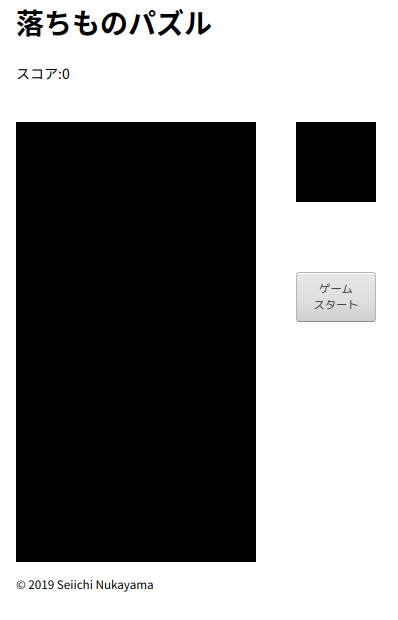
\includegraphics[width=6cm]{game1.png}

\end{document}

%% 修正時刻: Sat May  2 15:10:04 2020


%% 修正時刻: Sat Jun 20 22:03:18 2020
